\chapter{Conclusion}
\label{chapter:conclusion}

The Internet allows anyone to create content, publish and spread information. Social platforms are lowering the barrier of entry and are making it especially easy for everyone to have a voice on the Internet and as a result millions of messages and content of all forms is generated daily. Making sense of everything, and keeping track is becoming difficult and therefore it is time for tools that help understand the content to evolve and adapt to these mediums and make content exploration as easy as it is to post a message.
\newline
Dynamic applications such as social networks generate large amounts of text data and having an application capable of clustering and aggregating all the content is important for keeping track of events as news are more likely to be first reported in the online medium before others catch up.
\newline
The aim of this project was to build an application capable of clustering in real time streams of text generated by public messages from Twitter. Such a tool allows us to easily track news, trending topics or social media events as they occur and we can easily detect popular messages or common clusters of opinion.
\newline
{\project}  attempts to solve this problem of content discovery and exploration. {\project}  tracks the topics being published and presents it to the user in a way that is accessible and easy to use. It creates clusters of messages by interpreting content and presents it to the user in a web interface that allows for him to browse through a large number of messages efficiently.
\newline
The feature that makes {\project}  relevant for the fast passed rate of tweets is its ability to parse the messages in real time. The data is not based on an archived corpus of documents but on streaming tweets as they happen. This way popular events, news and messages get reported in the interface and the user is able to keep in touch with what is happening as events are taking place.
\newline
The goals we have set out for our project and managed to achieve:
\begin{itemize}
	\item Based on an input query, get real time messages from Twitter using its API.
	\item Parse tweets as they arrive: tokenize the sentences and using part-of-speech tagging to make annotations, help filter messages and extract important information.
	\item Cluster tweets efficiently. For this we chose K-Means algorithm which employs the meta information gathered in the previous step.
	\item Set up a decoupled system that can easily scale through the use of queues which allow for different rates of consumption and multiple consumers that can process the workload in parallel.
	\item Present the information through an accessible medium: the web browser, with an easy to use interface that allows the information to be explored.
\end{itemize}
Evaluating the results was done through calculating the purity coefficient for each cluster and thus computing internal coherence and by using the frontend {\frontend}. We expanded the clusters and started exploring the different topics making sure the results made sense.
One unexpected result that kept appearing in our experiments was discovering topic influencers. We define influencers as being people with large following in social media that also are really engaged with their followers through comments, retweets and favorites. The way it comes up in {\project}  is that a lot of people will end up retweeting a certain tweet written by one of these accounts, and it will show up as a cluster composed of the same tweet. There is also an exception, meaning that cluster can be composed of a single tweet of an account with few followers if their message was in turn retweeted by an influencer. In this case the cluster is formed entirely out of one popular tweet.
\newline
\begin{figure}[ht!]
\centering
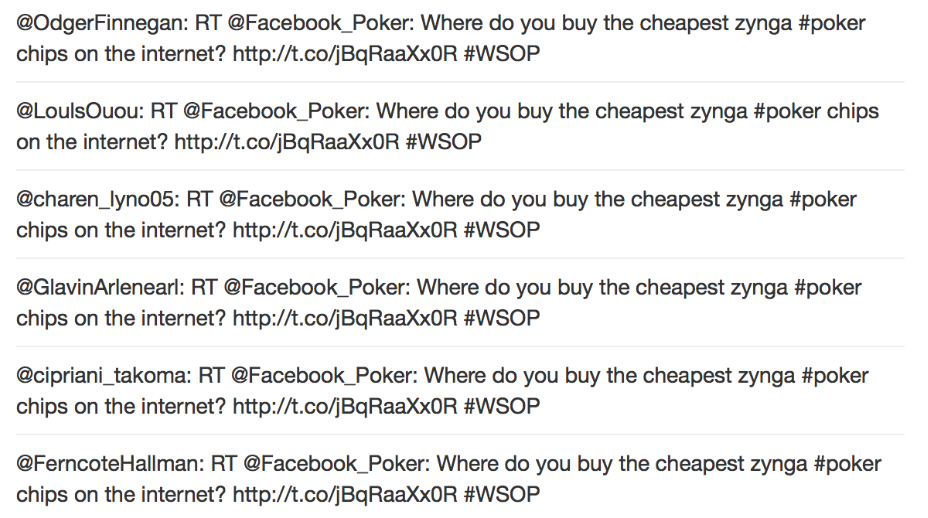
\includegraphics[width=\textwidth,height=\textheight,keepaspectratio]{src/img/bots.png}
\caption{Automated messages sent by bots\label{overflow}}
\end{figure}
\newline
Due to the way the Twitter stream API works: it sends a percentage of all tweets currently being exchanged that match your query, we were able to make another interesting observation. A large number of Twitter topic clusters are formed from messages from bots. Twitter bots produce automatic messages usually with spam or promotional links. For the topics we tested on, mostly programming language topics, we noticed a large number of clusters related to job advertisements which turned out to be automated messages.
\newline
In the figure we extracted an example of bot messages that are using a popular hashtag (World Series of Poker) to advertise a game. This also provides some indication that relying completely on hashtags in order to generate topics and cluster messages is not always very efficient. Bots might use trending topics to their advantage: most Twitter clients offer limited discovery features and usually just show tweets that match a certain hashtag, by using the same one, spam such as this can end up in your message list.
\newline
The application proved successful in clustering conversations, some of the topics we have experimented with were movies, receiving a wide variety of reviews from social media. Another such topic was programming languages where clusters usually grouped into ones containing tutorial links or job advertisements.
\newline
\newline
Having completed this initial first step, there are now potentially more areas where we can work on improving our project. Improvements both in terms of clustering and the information we highlight and present to the user. The following section \textbf{Future work} explores some of these ideas, what it would take to implement them and the benefits they would bring to the project.